%=====================================================================
\section{Model predictive control with the learned residual (RQ1)}\label{sec:mpc}
%=====================================================================
This section answers the control half of RQ1 and tests hypothesis \textbf{H3}: a residual Koopman MPC removes the steady error that model mismatch causes in a controller designed on the physics model (experiment E7).

\subsection{The MPC problem}
At every sample (5\,ms) the controller measures the current state, builds $\vect s_0 = (\vect x, \hat{\vect f})$ and solves
\begin{equation}\label{eq:mpc}
\begin{aligned}
\min_{\vect u_0,\dots,\vect u_{N-1}} \;& \textstyle\sum_{j=0}^{N-1}\big(\vect s_j^\top Q\,\vect s_j + \vect u_j^\top R\,\vect u_j\big) + \vect s_N^\top P_N\,\vect s_N\\
\text{subject to }\;& \vect s_{j+1} = A_d\vect s_j + B_d\vect u_j + \hat{\vect d},\qquad j = 0,\dots,N-1,\\
& f_{\min}-\bar f_i \;\le\; u_{j,i} \;\le\; f_{\max}-\bar f_i .
\end{aligned}
\end{equation}
\begin{itemize}
  \item The prediction model is the 10-state analytical model of Section~\ref{sec:koopman}.
  \item The horizon is $N = 20$ steps of 5\,ms, so the controller looks 100\,ms ahead.
  \item $Q$ and $R$ are the same weights as the failure LQR, so the two controllers aim for the same thing.
  \item The \emph{terminal cost} $P_N$ is the solution of the discrete-time Riccati equation for $(A_d, B_d, Q, R)$. It stands in for the cost after the horizon; with it, the MPC behaves like the discrete LQR whenever the limits are not active, which our tests check.
  \item The input limits are the motor thrust limits, written as deviations from the trim.
\end{itemize}
Only the first input $\vect u_0$ is applied; at the next sample the problem is solved again from the new measurement.

\subsection{Where the learned residual enters}
The \textbf{analytical MPC} uses $\hat{\vect d} = 0$. The \textbf{residual Koopman MPC} evaluates the learned residual once per sample, at the current state and previous input, \emph{outside} the optimization, and adds it to every predicted step as a known constant $\hat{\vect d}$ (a ``measured disturbance''), as Todde et al. do~\cite{todde2026residual}. The learned part is therefore not a decision variable, the constraints stay linear, and~\eqref{eq:mpc} stays a convex QP that solves reliably every time. The price is that the optimizer does not know how the residual would change with its own choice of inputs or along the predicted trajectory: the correction is frozen at its current value for the whole 100\,ms horizon.

\begin{plain}
The physics model plans the next 100\,ms; the learned residual tells it ``at the moment the real drone drifts this much more per step than you think'', and the plan compensates for that drift.
\end{plain}

\begin{codebox}{building and solving the QP once per sample}
\begin{lstlisting}
# built once: CVXPY parameters x0 and d, variables X (states) and U (inputs)
for j in range(N):
    cons += [X[:, j + 1] == Ad @ X[:, j] + Bd @ U[:, j] + self.d,
             U[:, j] >= lo, U[:, j] <= hi]
    cost += cp.quad_form(X[:, j], Q) + cp.quad_form(U[:, j], R)
cost += cp.quad_form(X[:, N], PN)                       # DARE terminal cost

# every sample
d[:7] = self.residual.residual(x7, self.fe, self.u_prev) # learned part, outside the QP
self.x0.value, self.d.value = np.concatenate((x7, self.fe)), d
self.prob.solve(solver=cp.OSQP, warm_start=True, eps_abs=1e-5, eps_rel=1e-5)
u = self.U.value[:, 0]                                   # apply the first move only
\end{lstlisting}
\end{codebox}
The problem is modelled with CVXPY~\cite{diamond2016cvxpy} and solved with OSQP~\cite{stellato2020osqp}, an operator-splitting QP solver; ``warm start'' reuses the previous solution as the starting guess.

\subsection{Experiment: steady altitude error under mismatch}
All three controllers (LQR, analytical MPC, residual Koopman MPC) are designed on the nominal parameters and flown on the mismatched truth plants. The residual is the one trained on family A in Section~\ref{sec:koopman}. Each run starts 1\,m below the set-point near the relaxed hover and lasts 8\,s; the steady error is the mean height over the last 2\,s. We use one run per plant and controller, because the steady state does not depend on the starting point. To see which effect causes the error, we also test each family without its thrust loss, and the nominal plant with only that family's thrust loss.

\begin{table}[h]
\centering\small
\caption{Steady altitude error near the relaxed hover (set-point 0\,m). The last column compares the \emph{magnitude} of the residual-MPC error with the LQR error; for plant B (full) the sign also changes.}\label{tab:mpc}
\begin{tabular}{lcccc}
\toprule
Plant & LQR & MPC, analytical & MPC, residual & Change \\
\midrule
A (full) & $-0.285$\,m & $-0.286$\,m & $\mathbf{-0.193}$\,m & $-32$\% \\
A without thrust loss & $-0.154$\,m & $-0.154$\,m & $-0.066$\,m & $-57$\% \\
Nominal + A's thrust loss only & $-0.100$\,m & $-0.101$\,m & $-0.033$\,m & $-67$\% \\
B (full, held out) & $-0.029$\,m & $-0.033$\,m & $+0.022$\,m & $-25$\% \\
B without thrust loss & $+0.112$\,m & $+0.111$\,m & $+0.164$\,m & $+47$\% \\
Nominal + B's thrust loss only & $-0.174$\,m & $-0.177$\,m & $-0.107$\,m & $-39$\% \\
\bottomrule
\end{tabular}
\end{table}

\begin{figure}[h]
\centering
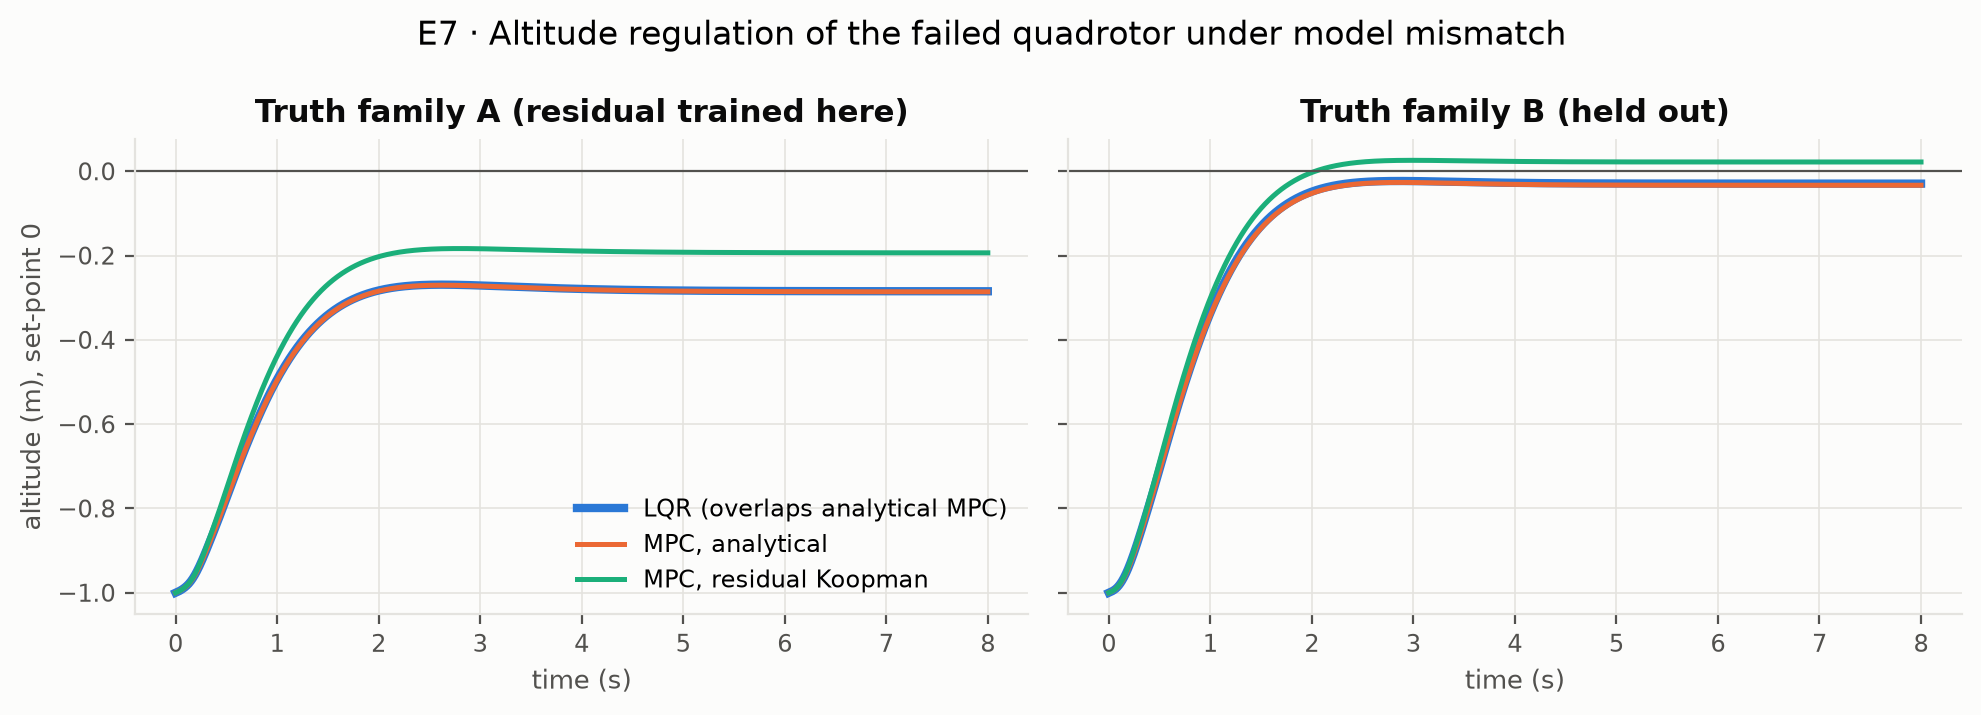
\includegraphics[width=\linewidth]{figures/e7_altitude.png}
\caption{Height of the failed drone under model mismatch for the three controllers (LQR and analytical MPC overlap). Left: family A, on which the residual was trained. Right: held-out family B.}\label{fig:mpc}
\end{figure}

\paragraph{Results.} On plant A, LQR and the analytical MPC both settle 0.29\,m too low; they are practically identical, because near the equilibrium the thrust limits are not reached and the MPC then acts like the LQR. The thrust loss alone causes 0.10\,m and the inertia and motor mismatch alone 0.15\,m; the effects are not exactly additive (together 0.29\,m). The residual Koopman MPC settles 0.19\,m low, a 32\% smaller error, and it reduces the error for each separate effect of plant A. On the held-out plant B the effects partly cancel. The residual MPC still reduces the error for the full plant and for its thrust loss alone, but when B's thrust loss is removed it makes the error 47\% \emph{larger}: the correction learned on A pushes in the wrong direction for that plant. This is the generalization problem of Section~\ref{sec:koopman} again. H3 is therefore only partly supported: on the training plant the error is reduced by 32\%, not removed, and on a held-out variant it grows. The errors on plant B are only a few centimetres, so their percentages should not be over-read.

The residual reduces the error but does not remove it. The classical way to remove a steady error caused by a constant mismatch is integral action, or an ``offset-free'' MPC that estimates a constant disturbance from the measurements; in theory it removes such an error completely. This is the most important missing baseline: until it is compared, the 32\% reduction shows that the residual carries useful information, not that it is the best way to remove the bias. A residual could still help where integral action is slow, for example during transients.

\paragraph{Computation time.} The QP solver needs a median of 0.73\,ms per sample. Through the CVXPY modelling layer the median wall-clock time is 4.4\,ms, which leaves almost no margin to the 5\,ms sample period. A real-time version would call the solver directly.
